\documentclass{article}
\usepackage{amsmath}
\usepackage{makeidx}
\usepackage{xcolor}
\usepackage{listings}
\usepackage{graphicx}
\usepackage{epstopdf}

\definecolor{mGreen}{rgb}{0,0.6,0}
\definecolor{mGray}{rgb}{0.5,0.5,0.5}
\definecolor{mPurple}{rgb}{0.58,0,0.82}
\definecolor{mBlack}{rgb}{0,0,0}
\definecolor{backgroundColour}{rgb}{0.95,0.95,0.92}

\lstdefinestyle{CStyle}{
    backgroundcolor=\color{backgroundColour},   
    commentstyle=\color{mGreen},
    keywordstyle=\color{magenta},
    numberstyle=\tiny\color{mGray},
    stringstyle=\color{mPurple},
    basicstyle=\footnotesize,
    breakatwhitespace=false,         
    breaklines=true,                 
    captionpos=b,                    
    keepspaces=false,                 
    numbers=none,                    
    numbersep=5pt,                  
    showspaces=false,                
    showstringspaces=false,
    showtabs=false,                  
    tabsize=2,
    frame=single,
    language=C
}

\lstdefinestyle{bashStyle}{
    backgroundcolor=\color{backgroundColour},   
    commentstyle=\color{mGreen},
    keywordstyle=\color{magenta},
    numberstyle=\tiny\color{mGray},
    stringstyle=\color{mPurple},
    basicstyle=\footnotesize,
    breaklines=true,
    language=bash
}

\begin{document}
\title{Practice linux kernal module}
\author{Danny Deng}
\date{Version 1.0}
\maketitle

\section{Command in terminal}

\textbf{See the command usage and information}
\begin{lstlisting}[style=bashStyle]
    $ man {command}
\end{lstlisting}
\text{Example:}
\begin{lstlisting}[style=bashStyle]
    $ man insmod
\end{lstlisting}
\text{Result}
\begin{center}
    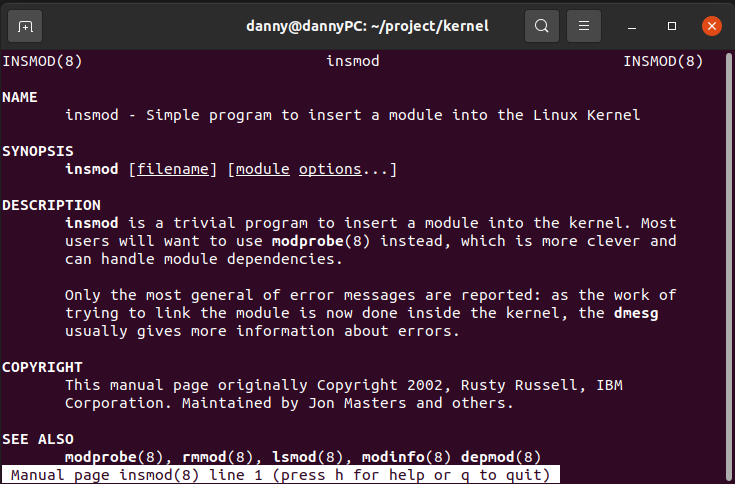
\includegraphics[width=\linewidth]{images/man_insmod.png}
\end{center}

\textbf{Insert a kernal module}
\begin{lstlisting}[style=bashStyle]
    $ sudo insmod {module name (*.ko)}
\end{lstlisting}

\textbf{Show a kernal module info}
\begin{lstlisting}[style=bashStyle]
    $ sudo modinfo {module name (*.ko)}
\end{lstlisting}

\textbf{Print or control the kernel ring buffer}
\begin{lstlisting}[style=bashStyle]
    $ sudo dmesg
\end{lstlisting}

\textbf{Simple program to remove a module from the Linux Kernel}
\begin{lstlisting}[style=bashStyle]
    $ sudo rmmod {module name}
\end{lstlisting}


\textbf{Add and remove modules from the Linux Kernel}

Loads the module only in /lib/modules/`uname -r`
modprobe depends on depmod tool to calculate dependancies
\begin{lstlisting}[style=bashStyle]
    $ sudo modprobe {module name}
    $ echo the dependancies
    $ vi /lib/module/`uname -r`/modules.dep
\end{lstlisting}










\section{Hello world}

\textbf{Example code below}
\begin{lstlisting}[style=CStyle]
    #include <linux/kernel.h>
    #include <linux/module.h>
    
    MODULE_LICENSE("GPL");
    static int test_hello_init(void) {
        printk(KERN_INFO"%s: In init \n", __func__);
        return 0;
    }
    
    static void test_hello_exit(void) {
        printk(KERN_INFO"%s: In exit \n", __func__);
    }
    
    module_init(test_hello_init);
    module_exit(test_hello_exit);    
\end{lstlisting}

\textbf{Include header and define the LICENSE(option)}
\begin{lstlisting}[style=CStyle]
#include <linux/kernel.h>
#include <linux/module.h>

MODULE_LICENSE("GPL");
\end{lstlisting}

\textbf{When insert module, it will call the initial function}
\begin{lstlisting}[style=CStyle]
    static int test_hello_init(void) {
        printk(KERN_INFO"%s: In init \n", __func__);
        return 0;
    }

    module_init(test_hello_init);
\end{lstlisting}

\textbf{When rmmod the kernel module, it will call the exit function}
\begin{lstlisting}[style=CStyle]
    static void test_hello_exit(void) {
        printk(KERN_INFO"%s: In exit \n", __func__);
    }

    module_exit(test_hello_exit);
\end{lstlisting}


\textbf{Build steps}
\begin{enumerate}
    \item Write the Makefile
\begin{lstlisting}[style=bashStyle]
obj-m := hello_world.o

all:
    make -C /lib/modules/`uname -r`/build M=${PWD} modules

clean:
    make -C /lib/modules/`uname -r`/build M=${PWD} clean
\end{lstlisting}
    \item Build
\begin{lstlisting}[style=bashStyle]
    $ make all
\end{lstlisting}
\end{enumerate}



\section{Passing parameters to linux kernel module}

\text{Using \textit{module\_param} function to declare parameters}

\textbf{Example code below}
\begin{lstlisting}[style=CStyle]
    #include <linux/kernel.h>
    #include <linux/module.h>
    
    MODULE_LICENSE("GPL");
    
    char *name = "Danny";
    int count = 0;
    module_param(name, charp, S_IRUGO);
    module_param(count, int, S_IRUGO);
    
    
    static int test_arguments_init(void) {
        printk(KERN_INFO"%s: In init\n", __func__);
        printk(KERN_INFO"%s: name: %s\n", __func__, name);
        printk(KERN_INFO"%s: pass count: %d\n", __func__, count);
    
        return 0;
    }
    
    
    static void test_exit(void) {
        printk(KERN_INFO"%s: In exit: \n", __func__);
    }
    
    
    
    module_init(test_arguments_init);
    module_exit(test_exit);
    
    MODULE_AUTHOR("Danny Deng");
    MODULE_DESCRIPTION("Argument parsing example");    
\end{lstlisting}

\text{}

\textbf{Each parameters can declare different permission}
\begin{center}
    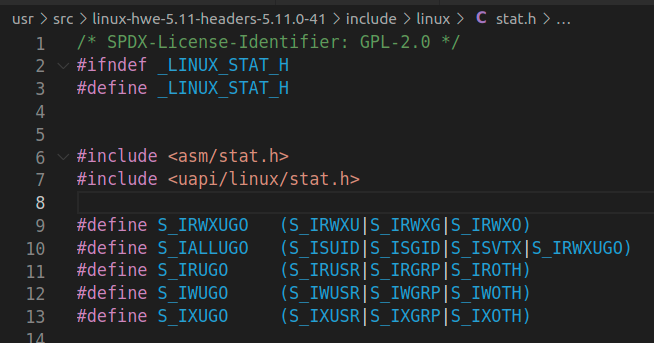
\includegraphics[width=\linewidth]{images/kernel_permission.png}
\end{center}

\textbf{The macro value define below}
\begin{lstlisting}[style=CStyle]
#define S_IRWXU 00700
#define S_IRUSR 00400
#define S_IWUSR 00200
#define S_IXUSR 00100

#define S_IRWXG 00070
#define S_IRGRP 00040
#define S_IWGRP 00020
#define S_IXGRP 00010

#define S_IRWXO 00007
#define S_IROTH 00004
#define S_IWOTH 00002
#define S_IXOTH 00001
\end{lstlisting}

\text{S\_I + R/W/X + USR/GRP/OTH}
\begin{itemize}
    \item R: Read
    \item W: Write
    \item X: Execute
    \item USR: User
    \item GRP: Group
    \item OTH: Other
\end{itemize}

\textbf{Insert the kernel module, and feed the parameter}
\begin{lstlisting}[style=bashStyle]
    $ sudo insmod passing_simple_count.ko count=10 name=Danny
\end{lstlisting}

\textbf{Remove the kernel module}
\begin{lstlisting}[style=bashStyle]
    $ sudo rmsmod passing_simple_count
\end{lstlisting}

\textbf{Show the result}
\begin{lstlisting}[style=bashStyle]
    $ dmesg
\end{lstlisting}

\begin{center}
    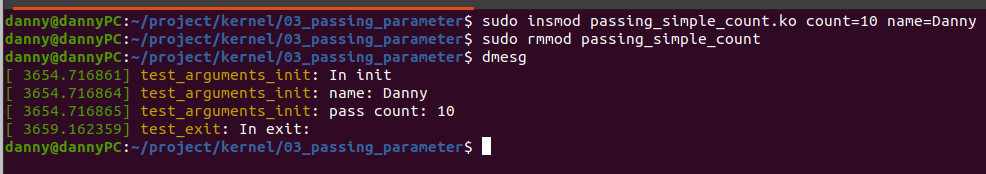
\includegraphics[width=\linewidth]{images/03_pass_para_terminal.png}
\end{center}





% \printindex
\end{document}
